% !TeX spellcheck = pl_PL
\documentclass[10pt, xcolor={dvipsnames,svgnames}, aspectratio=169]{beamer}
\usepackage{beamerthemeiitisask}
\usepackage{fontawesome}
\usepackage{qrcode}
\usepackage{circuitikz}
\usepackage{qcircuit}
\usepackage{listings}
\usepackage{tikz}
\usepackage{overpic}

\usepackage{hyperref}
\usepackage{subcaption}
\usepackage{tabularx}
\usepackage{multirow}
\usepackage[export]{adjustbox}
\usepackage{mathbbol}

\usepackage[lined]{algorithm2e}
\usepackage{comment}
\usepackage{stmaryrd}
\usepackage{tabularx}
% ------------------------------------------------------------------ %
\begin{document}
\title{Kwantowe uczenie maszynowe i kwantowe metody jądrowe}
\author{Piotr Gawron}
\date{}
\frame{\maketitle}
\include{lecture_1_introduction.tex}
\section{Gate model of computation}
%%%%%%%%%%%%%%%%%%%%%%%%%%%%%%%%%%%%%%%%%%%%%%%%%%%%%%%%%%%%%%%%%%%%%%%%%%%%%%%%
\begingroup
\nologo
\begin{frame}{Gate model}
\begin{block}{How to perform computations?}
\begin{itemize}
\item Prepare the system in a known state, eg.: $\ket{0} \otimes \ket{1}$.
\item Apply quantum gates and partial measurements on the state.
\item Perform the measurement.
\item Analyze the result and post-processing. 
\end{itemize}
\end{block}
\vspace{0.5cm}
\begin{block}{Example of a quantum circuit}
\begin{figure}
\centering
\mbox{
\Qcircuit @C=1em @R=.7em { 
\lstick{\ket{0}} & \qw & \gate{H}  & \qw & \multigate{1}{U_f} & \qw 
& \gate{H} & \qw & \meter & \cw 
\\ 
\lstick{\ket{1}} & \qw & \gate{H} & \qw & \ghost{U_f} & \qw 
& \qw & \qw & \qw &  \qw 
}
}
\end{figure}
\end{block}
\end{frame}
\endgroup%%%%%%%%%%%%%%%%%%%%%%%%%%%%%%%%%%%%%%%%%%%%%%%%%%%%%%%%%%%%%%%%%%%%%%%%%%%%%%%%
\subsection{Classical gates}
%%%%%%%%%%%%%%%%%%%%%%%%%%%%%%%%%%%%%%%%%%%%%%%%%%%%%%%%%%%%%%%%%%%%%%%%%%%%%%%%
\begin{frame}{Classical gates}
\begin{columns}
\begin{column}[c]{0.5\textwidth}
\begin{circuitikz}[]
% something does not work here!
\node[buffer port] (BUF) at (0,0){};
\draw (BUF.out) -- ++(0.6,0) node[near end,above](Out){$x$};
\draw (BUF.in) -- ++(-0.2,0)node[left](In){$x$};
\end{circuitikz}\\[1cm]
\begin{circuitikz}[]
\node[not port] (NOT) at (0,0){};
\draw (NOT.out) -- ++(0.6,0) node[near end,above](Out){$\neg 
x$};
\draw (NOT.in) -- ++(-0.2,0)node[left](In){$x$};
\end{circuitikz}
\end{column}
\begin{column}[c]{0.5\textwidth}
\begin{circuitikz}[]
\node[or port] (OR) at (0,0){};
\draw (OR.out) -- ++(0.6,0) node[near end,above](Out){$x \text{ 
OR } y$};
\draw (OR.in 1) -- ++(-0.2,0)node[left](In1){$x$};
\draw (OR.in 2) -- ++(-0.2,0)node[left](In2){$y$};
\end{circuitikz}\\[1cm]
\begin{circuitikz}[]
\node[and port] (AND) at (0,0){};
\draw (AND.out) -- ++(0.6,0) node[near end,above](Out){$x 
\text{ AND } y$};
\draw (AND.in 1) -- ++(-0.2,0)node[left](In1){$x$};
\draw (AND.in 2) -- ++(-0.2,0)node[left](In2){$y$};
\end{circuitikz}\\[1cm]
\begin{circuitikz}[]
\node[xor port] (XOR) at (0,0){};
\draw (XOR.out) -- ++(0.6,0) node[near end,above](Out){$x 
\oplus y$};
\draw (XOR.in 1) -- ++(-0.2,0)node[left](In1){$x$};
\draw (XOR.in 2) -- ++(-0.2,0)node[left](In2){$y$};
\end{circuitikz}
\end{column}
\end{columns}
\end{frame}
%%%%%%%%%%%%%%%%%%%%%%%%%%%%%%%%%%%%%%%%%%%%%%%%%%%%%%%%%%%%%%%%%%%%%%%%%%%%%%%%
\subsection{Single qubit gates}
%%%%%%%%%%%%%%%%%%%%%%%%%%%%%%%%%%%%%%%%%%%%%%%%%%%%%%%%%%%%%%%%%%%%%%%%%%%%%%%%
\begin{frame}{Single qubit gate --- unitary gate}
\begin{block}{How to denote a quantum single-qubit gate?}
\vspace{0.5cm}
\centering

\begin{tabular}{c c c}
$\ket{\psi}$ &
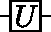
\includegraphics[valign=m, scale=1]{pics/unitary} &   $U \ket\psi$
\end{tabular}
\end{block}

\vspace{1cm}
\begin{block}{Quantum evolution is time-reversible!}
\begin{equation*}
U\ket{\psi_{t=0}} = \ket{\psi_{t=1}}
\end{equation*}
\begin{equation*}
U^\dagger\ket{\psi_{t=1}} = \ket{\psi_{t=0}}
\end{equation*}
\end{block}
\end{frame}
%%%%%%%%%%%%%%%%%%%%%%%%%%%%%%%%%%%%%%%%%%%%%%%%%%%%%%%%%%%%%%%%%%%%%%%%%%%%%%%%
\begin{frame}{Rotations}
\begin{columns}
\begin{column}[t]{0.35\textwidth}
\begin{center}
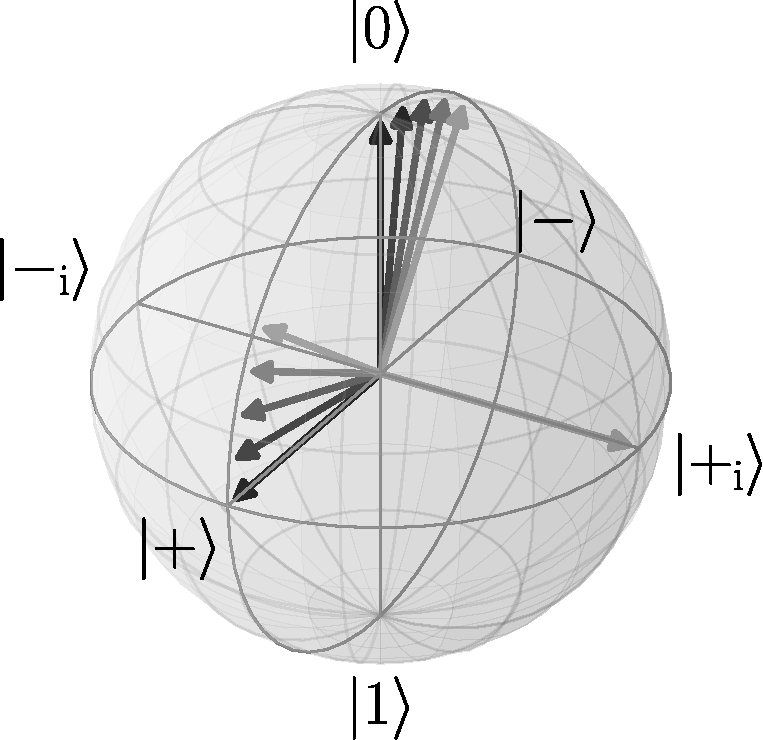
\includegraphics[width=0.8\textwidth]{pics/Ry} \\
$$
R_y(\gamma) = 
\begin{bmatrix}
\cos\left(\frac{\gamma}{2}\right) & \sin\left(\frac{\gamma}{2}\right)         \\
-\sin\left(\frac{\gamma}{2}\right) & \cos\left(\frac{\gamma}{2}\right)
\end{bmatrix}
$$
\end{center}
\end{column}
% \vrule{}
\begin{column}[t]{0.35\textwidth}
\begin{center}
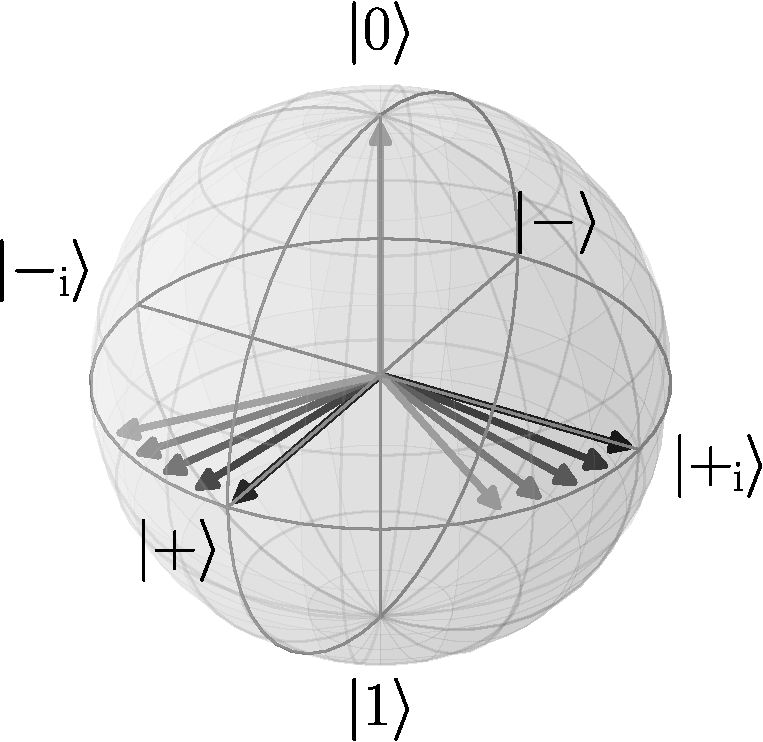
\includegraphics[width=0.8\textwidth]{pics/Rz} \\
$$
R_z(\beta) = 
\begin{bmatrix}
\mathrm{e}^{\frac{\mathrm{i} \beta}{2}} & 0        \\
0 & - \mathrm{e}^{\frac{\mathrm{i} \beta}{2}}
\end{bmatrix}
$$
\end{center}
\end{column}
\end{columns}
\end{frame}
%%%%%%%%%%%%%%%%%%%%%%%%%%%%%%%%%%%%%%%%%%%%%%%%%%%%%%%%%%%%%%%%%%%%%%%%%%%%%%%%
\begin{frame}{Important examples of single-qubit gates}
\centering
\begin{tabularx}{0.65\textwidth}{Xc}
\parbox[c]{\hsize}{
	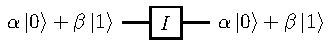
\includegraphics[page=1]{pics/single_qubit_gates.pdf}
} &
$
\begin{bmatrix}
1 & 0 \\
0 & 1
\end{bmatrix}
$
\\ [0.8cm]
\parbox[c]{\hsize}{
	\includegraphics[page=2]{pics/single_qubit_gates.pdf}
} &
$
\begin{bmatrix}
0 & 1 \\
1 & 0
\end{bmatrix}
$
\\[0.8cm]
\parbox[c]{\hsize}{
	\includegraphics[page=3]{pics/single_qubit_gates.pdf}
} &
$
\begin{bmatrix}
0 & -\mathrm{i}  \\
\mathrm{i} & 0
\end{bmatrix}
$
\\ [0.8cm]
\parbox[c]{\hsize}{
	\includegraphics[page=4]{pics/single_qubit_gates.pdf}
} &
$
\begin{bmatrix}
1 & 0         \\
0 & -1
\end{bmatrix}
$
\\ [0.8cm]
\parbox[c]{\hsize}{
	\includegraphics[page=5]{pics/single_qubit_gates.pdf}
} &
$
\begin{bmatrix}
1 & 0         \\
0 & \mathrm{e}^{\mathrm{i} \phi}
\end{bmatrix}
$
\end{tabularx}
\end{frame}

\begin{frame}{Hadamard gate}
\centering
$
H= \frac{1}{\sqrt{2}}\begin{bmatrix}
1 & 1         \\
1 & -1
\end{bmatrix},
$
\quad
$H\ket{0}=\frac{\ket{0}+\ket{1}}{\sqrt{2}}$, 
\quad
$H\ket{1}=\frac{\ket{0}-\ket{1}}{\sqrt{2}}$.
\\
\vspace{0.5cm}
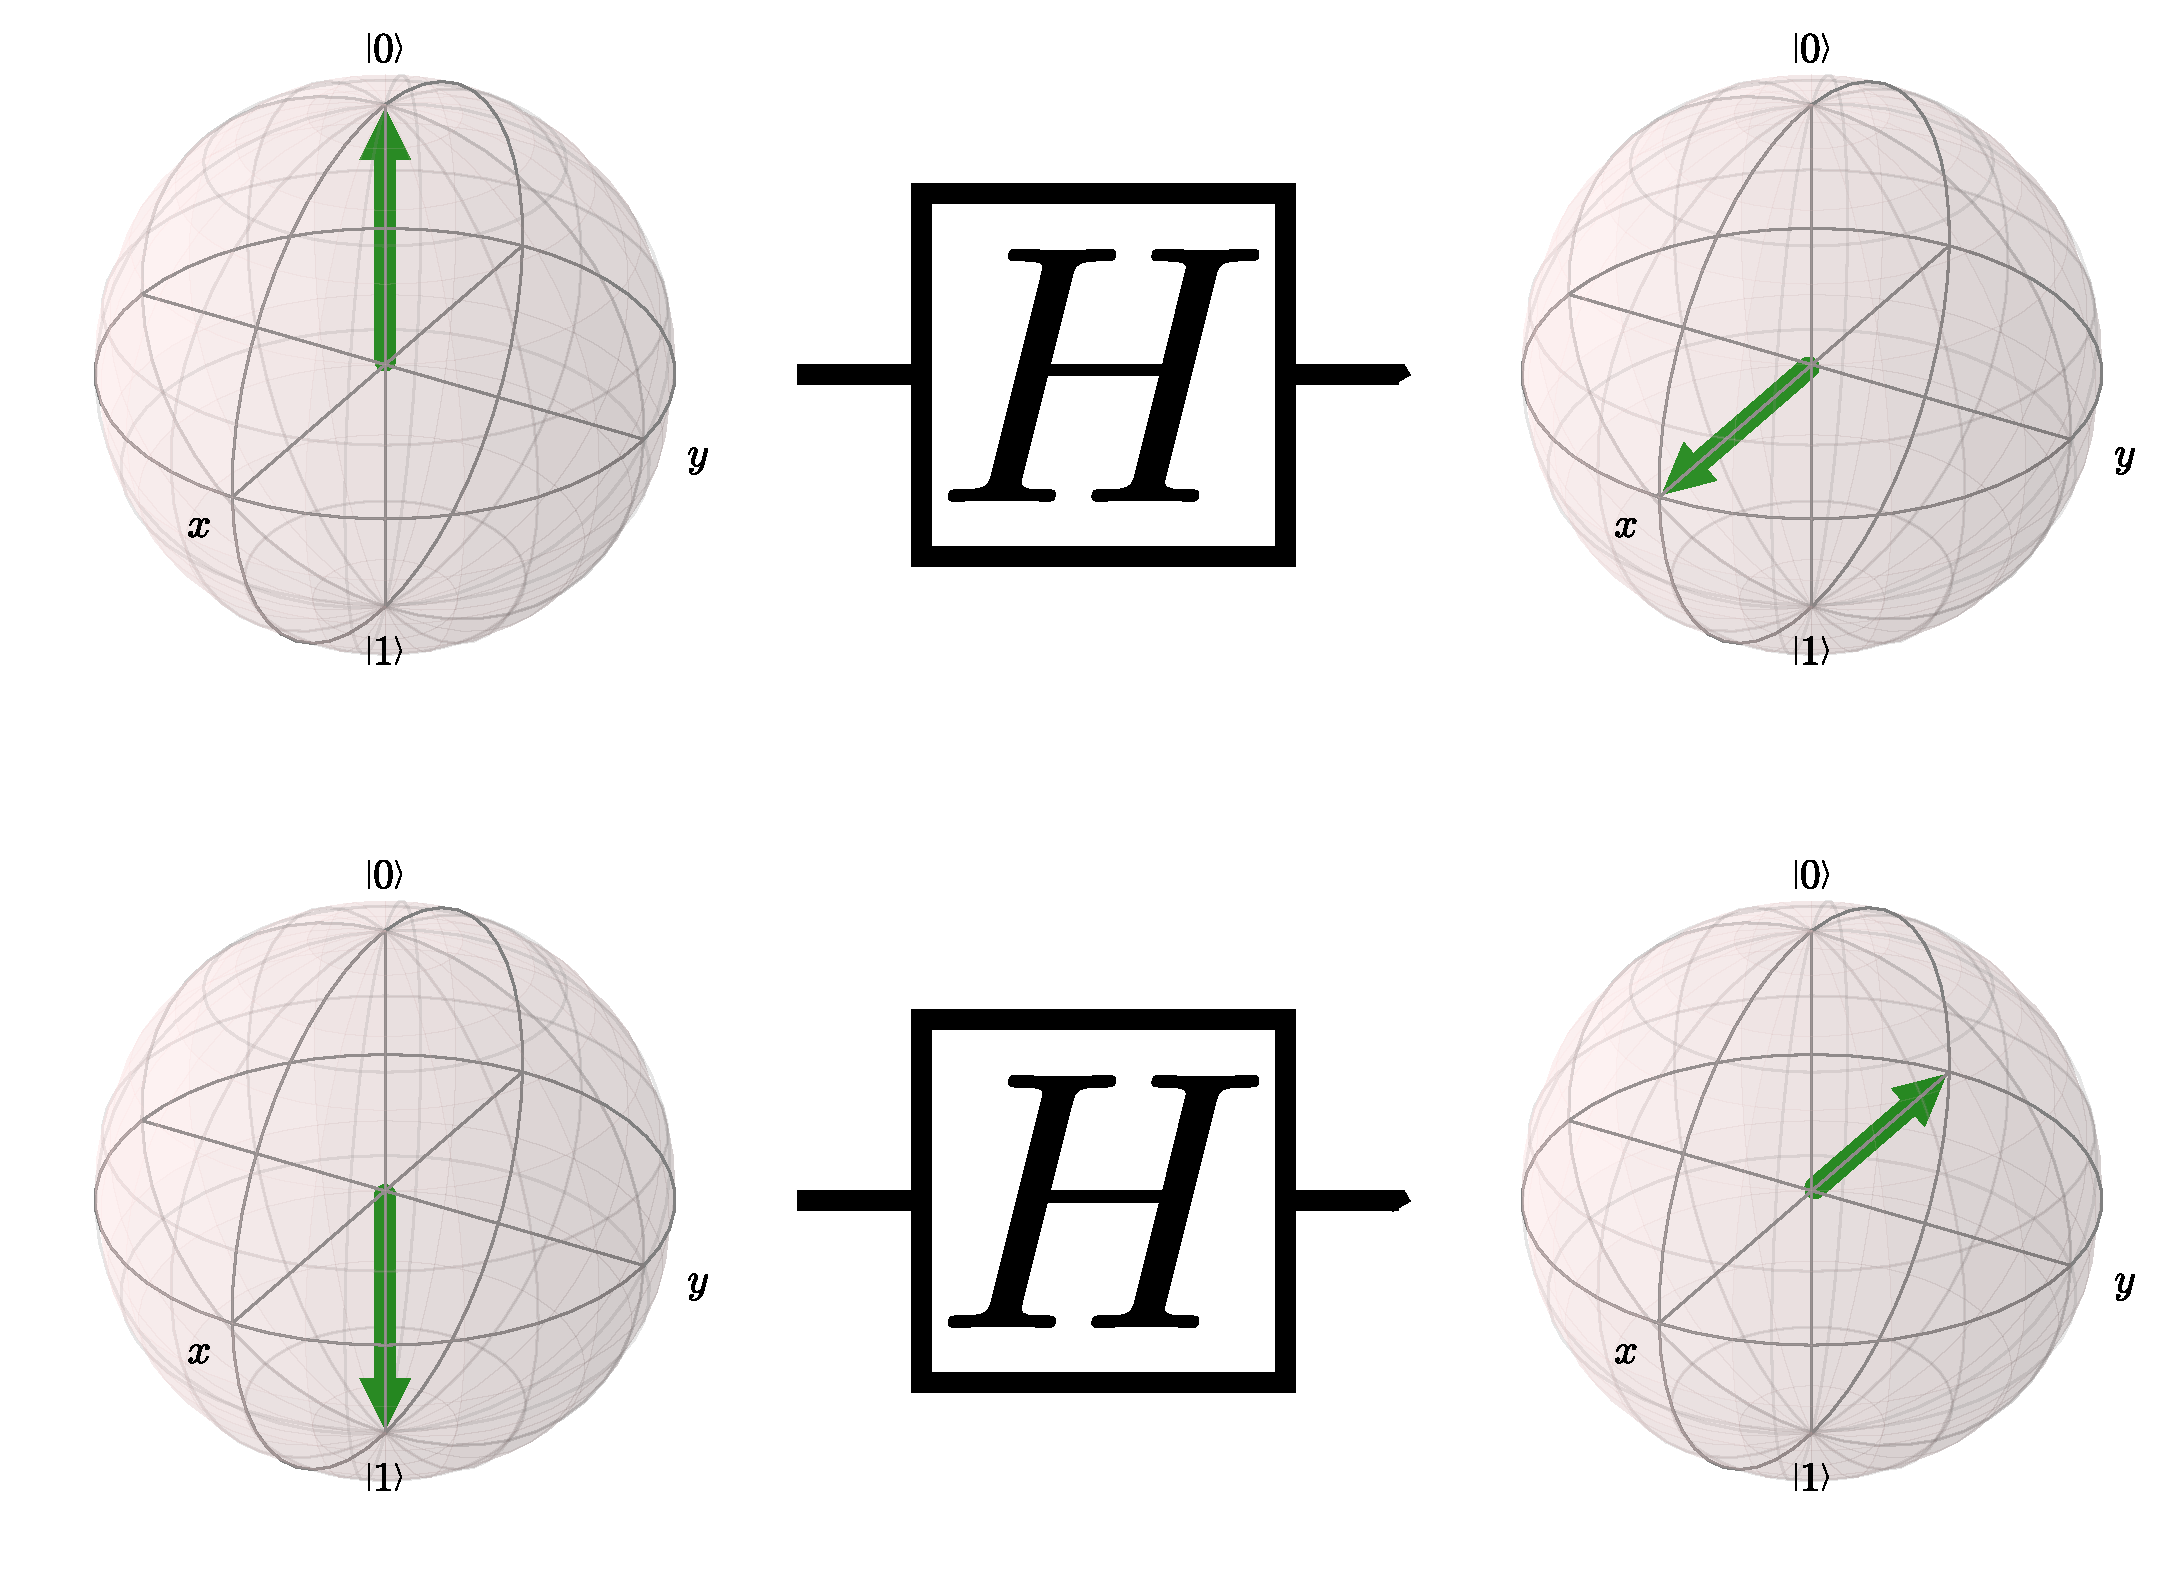
\includegraphics[width=0.5\textwidth]{pics/ewolucja}
\end{frame}

% % % % % % % % % % % % %

\begin{frame}{Decomposition of a unitary gate}
\begin{block}{Definition}
A square matrix is called \emph{unitary} iff 
\begin{equation*}
U U^\dagger = U^\dagger U = \mathbb{1}.
\end{equation*} 
\end{block}
\begin{block}{Every unitary gate $U$ can be written as}
\centering
%\begin{tabular}{c|c|c}
%UNITARY &
%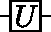
\includegraphics[valign=m, scale=1]{pics/unitary} &
%$U\ket{\psi_1} = \ket{\psi_2}$, $U^\dagger\ket{\psi_2} = \ket{\psi_1}$
%\end{tabular}
%\begin{figure}
%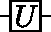
\includegraphics[valign=m, scale=1]{pics/unitary}
%\end{figure}

$$U = R_Z(\psi) R_Y (\theta) R_Z(\Delta)
=e^{i\varphi /2}{\begin{bmatrix}e^{i\psi }&0\\0&e^{-i\psi 
}\end{bmatrix}}{\begin{bmatrix}\cos \theta &\sin \theta \\-\sin \theta &\cos 
\theta \\\end{bmatrix}}{\begin{bmatrix}e^{i\Delta }&0\\0&e^{-i\Delta 
}\end{bmatrix}}.$$
\end{block}
\end{frame}

\begin{frame}{CNOT gate}
%\begin{block}{}
\centering
\begin{tabular}{c c}
%CNOT &
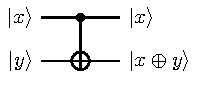
\includegraphics[valign=c,page=1,scale=1.1]{pics/two_qubit_gates.pdf} &
%
\includegraphics[valign=b, scale=2]{pics/cnot} &
\begin{tabular}{cc|cc}
$\text{in}_1$ & $\text{in}_2$ & $\text{out}_1$ & $\text{out}_2$ \\
\hline
0 & 0 & 0 & 0\\
0 & 1 & 0 & 1\\
1 & 0 & 1 & 1\\
1 & 1 & 1 & 0 
\end{tabular}
\end{tabular}
%\end{block}

\vspace{1.5cm}
\begin{tabularx}{\textwidth}{Xc}
\centering
%\parbox[c]{\hsize}{
%%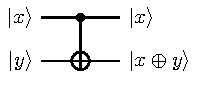
\includegraphics[page=1]{pics/two_qubit_gates.pdf}
%} &
$
\begin{bmatrix}
	1 & 0 & 0 & 0 \\
	0 & 1 & 0 & 0 \\
	0 & 0 & 0 & 1 \\
	0 & 0 & 1 & 0
\end{bmatrix}:
\begin{bmatrix}
	\alpha \\
	\beta  \\
	\gamma \\
	\delta
\end{bmatrix} \to
\begin{bmatrix}
	\alpha \\
	\beta  \\
	\delta \\
	\gamma
\end{bmatrix}
$
\end{tabularx}
\end{frame}

\begin{frame}{Controlled unitary}
%\begin{block}{}
\begin{tabularx}{0.8\textwidth}{Xc}

\parbox[c]{\hsize}{
\begin{figure}
\centering
\mbox{
\Qcircuit @C=2em @R=1em { 
 & \ctrl{1} & \qw \\ 
& \gate{U} & \qw }
}
\end{figure}
}
&
$
U=
\begin{bmatrix}
u_{00} & u_{01} \\
u_{10} & u_{11}
\end{bmatrix}
$
\end{tabularx}
%\end{block}
\vspace{0.8cm}

%\begin{block}{}
\begin{tabularx}{\textwidth}{Xc}
\centering
$
CU_1^2 =  \ketbra{0}{0} \otimes \mathbb{I} + 
\ketbra{1}{1} \otimes U = 
\begin{bmatrix}
	1 & 0 & 0 & 0 \\
	0 & 1 & 0 & 0 \\
	0 & 0 & u_{00} & u_{01} \\
	0 & 0 & u_{10} & u_{11}
\end{bmatrix}
$
\end{tabularx}
%\end{block}

\end{frame}


\subsection{2-qubit gates}
%%%%%%%%%%%%%%%%%%%%%%%%%%%%%%%%%%%%%%%%%%%%%%%%%%%%%%%%%%%%%%%%%%%%%%%%%%%%%%%%
\begin{frame}{Swap gate}
\centering
\begin{tabularx}{0.8\textwidth}{Xc}
%\parbox[c]{\hsize}{
%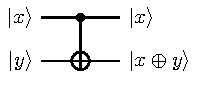
\includegraphics[page=1]{pics/two_qubit_gates.pdf}
%} &
%$
%\begin{bmatrix}
%	1 & 0 & 0 & 0 \\
%	0 & 1 & 0 & 0 \\
%	0 & 0 & 0 & 1 \\
%	0 & 0 & 1 & 0
%\end{bmatrix}:
%\begin{bmatrix}
%	\alpha \\
%	\beta  \\
%	\gamma \\
%	\delta
%\end{bmatrix} \to
%\begin{bmatrix}
%	\alpha \\
%	\beta  \\
%	\delta \\
%	\gamma
%\end{bmatrix}
%$   \\[0.8cm]
\parbox[c]{\hsize}{
\includegraphics[page=2]{pics/two_qubit_gates.pdf}
}
&
$
\begin{bmatrix}
	1 & 0 & 0 & 0 \\
	0 & 0 & 1 & 0 \\
	0 & 1 & 0 & 0 \\
	0 & 0 & 0 & 1
\end{bmatrix}:
\begin{bmatrix}
	\alpha \\
	\beta  \\
	\gamma \\
	\delta
\end{bmatrix} \to
\begin{bmatrix}
	\alpha \\
	\gamma \\
	\beta  \\
	\delta
\end{bmatrix}
$   \\[1.8cm]
\parbox[c]{\hsize}{
\includegraphics[page=3]{pics/two_qubit_gates.pdf}
}
&
$
\begin{bmatrix}
	1 & 0             & 0             & 0 \\
	0 & \frac{1+i}{2} & \frac{1-i}{2} & 0 \\
	0 & \frac{1-i}{2} & \frac{1+i}{2} & 0 \\
	0 & 0             & 0             & 1
\end{bmatrix}:
\begin{bmatrix}
	\alpha \\
	\beta  \\
	\gamma \\
	\delta
\end{bmatrix} \to
\begin{bmatrix}
	\alpha                                   \\
	\frac{1+i}{2}\beta + \frac{1-i}{2}\gamma \\
	\frac{1-i}{2}\beta + \frac{1+i}{2}\gamma \\
	\delta
\end{bmatrix}
$
\end{tabularx}
\end{frame}

\begin{frame}{Example of a circuit}
\begin{figure}
\centering
\mbox{
\Qcircuit @C=1em @R=.7em { 
\lstick{\ket{0}} & \qw & \gate{H}  & \qw &\ctrl{1} & \qw \\
\lstick{\ket{0}} & \qw & \qw  & \qw  & \targ & \qw
}
}
\end{figure}
%\centering
% 
\includegraphics[page=1]{pics/example_of_quantum_circuit.pdf}
\begin{enumerate}
\item $(H \otimes I)\ket{0} \otimes \ket{0} =
\frac{1}{\sqrt{2}} \left( \ket{0} + \ket{1} \right) \otimes \ket{0}
= 
\frac{1}{\sqrt{2}}
\begin{bmatrix}
1 \\
0 \\
1 \\
0
\end{bmatrix}
$

\item
$ \begin{bmatrix}
	1 & 0 & 0 & 0 \\
	0 & 1 & 0 & 0 \\
	0 & 0 & 0 & 1 \\
	0 & 0 & 1 & 0
\end{bmatrix}
%\frac{1}{\sqrt{2}}
\begin{bmatrix}
\frac{1}{\sqrt{2}} \\
0 \\
\frac{1}{\sqrt{2}} \\
0
\end{bmatrix}
= 
\begin{bmatrix}
\frac{1}{\sqrt{2}} \\
0 \\
0 \\
\frac{1}{\sqrt{2}} 
\end{bmatrix}
= \frac{1}{\sqrt{2}} \left(  \ket{00} + \ket{11} \right)
$
\end{enumerate}
\end{frame}

\include{lecture_2_gate_model_b.tex}
\include{lecture_3_qml.tex}

\end{document}